\section{Лекция 5. Методы интегрирования дифференциальных уравнений 1-го порядка}
\noeqref{eq:l5_hom_def, eq:l5_hom_ode1, eq:l5_hom_ode2, eq:l5_subst}
\noeqref{eq:l5_subst_der, eq:l5_sep_z, eq:l5_ex1, eq:l5_red_hom}
\noeqref{eq:l5_red_sys, eq:l5_red_subst, eq:l5_ex2, eq:l5_par_subst}
\noeqref{eq:l5_par_der, eq:l5_par_sep, eq:l5_ex_par}

\begin{flushright}
    05.10.26
\end{flushright}

\subsection{Роль уравнений с разделяющимися переменными}

В Лекции 2 (раздел 2.1) мы подробно изучили уравнения с разделяющимися
переменными вида $y' = P(x) \cdot Q(y)$, где $P \in C(I_x)$ и $Q \in C(I_y)$.
Напомним ключевое правило: при делении на $Q(y)$ для разделения переменных
необходимо отдельно проверять стационарные корни уравнения $Q(y) = 0$ на
предмет потери решений.

Этот класс уравнений служит фундаментом аналитической теории ОДУ 1-го порядка:
интегрирование большинства других классов уравнений (однородных, приводящихся
к однородным, обобщённо-однородных, линейных и уравнения Бернулли) основано на
поиске замены переменных, сводящей исходную задачу к уравнению с
разделяющимися переменными.

\subsection{Однородные дифференциальные уравнения}

Введём предварительно алгебраическое понятие однородной функции двух
переменных.

\begin{definition}
    Функция $f(x, y)$ называется \textdef{однородной функцией измерения
    (порядка) $k \in \R$}, если для любого $\lambda > 0$ (или
    $\lambda \in \R \setminus \{0\}$) и любой точки $(x, y)$ из области
    определения выполняется тождество:
    \begin{equation} \label{eq:l5_hom_def}
        f(\lambda x, \lambda y) = \lambda^k f(x, y). \tag{1}
    \end{equation}
\end{definition}

\begin{example}
    Рассмотрим функцию $f(x, y) = x^2 - x y + 2 y^2$. Подставим $\lambda x$ и
    $\lambda y$:
    \[
        f(\lambda x, \lambda y) = (\lambda x)^2 - (\lambda x)(\lambda y) +
        2(\lambda y)^2 = \lambda^2 \left(x^2 - x y + 2 y^2\right) =
        \lambda^2 f(x, y).
    \]
    Следовательно, данная функция является однородной измерения $k = 2$.
\end{example}

\begin{definition}
    \textdef{Однородным дифференциальным уравнением} 1-го порядка называется
    уравнение, которое можно записать в виде:
    \begin{equation} \label{eq:l5_hom_ode1}
        y' = f\left(\frac{y}{x}\right), \tag{2}
    \end{equation}
    где $f \in C(I)$, или в симметричной дифференциальной форме:
    \begin{equation} \label{eq:l5_hom_ode2}
        P(x, y) \, dx + Q(x, y) \, dy = 0, \tag{3}
    \end{equation}
    где $P(x, y)$ и $Q(x, y)$ — непрерывные однородные функции \textbf{одного
    и того же измерения $k$}.
\end{definition}

\textbf{Геометрический смысл однородного ОДУ:}
Поскольку правая часть уравнения \eqref{eq:l5_hom_ode1} зависит только от
отношения $y/x$, изоклинами $\frac{y}{x} = k = \text{const}$ служат лучи
(прямые $y = k x$), выходящие из начала координат. Поэтому поле направлений
инвариантно относительно преобразования подобия (гомотетии) с центром в точке
$(0, 0)$: если кривая $\gamma$ является интегральной, то при растяжении в
$\lambda$ раз получается также интегральная кривая.

\begin{figure}[H]
    \centering
    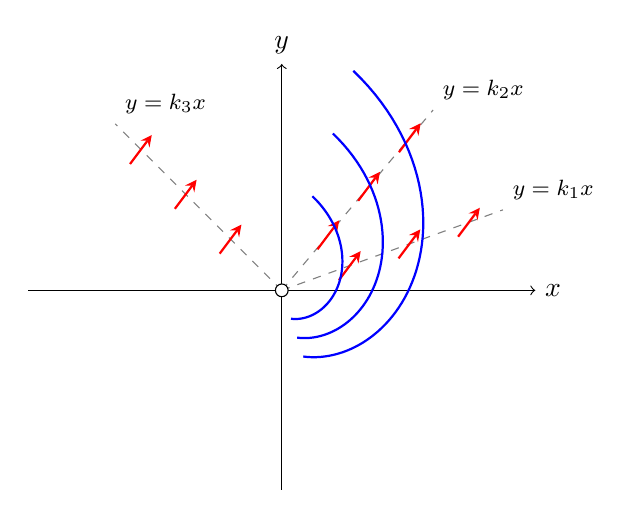
\begin{tikzpicture}[scale=1.15]
        % Оси координат
        \draw[->] (-2.8, 0) -- (2.8, 0) node[right] {$x$};
        \draw[->] (0, -2.2) -- (0, 2.5) node[above] {$y$};

        % Лучи-изоклины y = k x
        \foreach \ang/\lbl in {20/k_1, 50/k_2, 135/k_3} {
            \draw[dashed, gray] (0, 0) -- (\ang:2.6)
                node[above right, black] {\footnotesize $y = \lbl x$};
            \foreach \r in {0.8, 1.5, 2.2} {
                \pgfmathsetmacro{\px}{\r * cos(\ang)}
                \pgfmathsetmacro{\py}{\r * sin(\ang)}
                \draw[red, thick, -stealth]
                    (\px - 0.12, \py - 0.16) -- (\px + 0.12, \py + 0.16);
            }
        }

        % Гомотетичные интегральные кривые
        \foreach \s in {0.6, 1.0, 1.4} {
            \draw[blue, thick, domain=-1.2:1.2, samples=60]
                plot ({\s * exp(0.5*\x) * cos(60*\x)},
                      {\s * exp(0.5*\x) * sin(60*\x)});
        }
        \fill[white] (0, 0) circle (2pt);
        \draw[black] (0, 0) circle (2pt);
    \end{tikzpicture}
    \caption{Геометрическая интерпретация однородного уравнения: изоклинами
    являются прямые $y = k x$, проходящие через начало координат, а
    интегральные кривые переходят друг в друга при гомотетии.}
\end{figure}

\begin{proof}[Метод интегрирования однородного уравнения]~\\
    \begin{quote}
        Введём новую неизвестную функцию $z = z(x)$ по формуле:
        \begin{equation} \label{eq:l5_subst}
            z(x) = \frac{y}{x} \iff y = z \cdot x. \tag{4}
        \end{equation}
        Дифференцируя произведение по $x$, получаем:
        \begin{equation} \label{eq:l5_subst_der}
            y' = z' x + z. \tag{5}
        \end{equation}
        Подставим соотношения \eqref{eq:l5_subst} и \eqref{eq:l5_subst_der} в
        уравнение \eqref{eq:l5_hom_ode1}:
        \[
            z' x + z = f(z) \implies x \frac{dz}{dx} = f(z) - z.
        \]
        Мы пришли к уравнению с разделяющимися переменными относительно
        $z(x)$:
        \begin{equation} \label{eq:l5_sep_z}
            \frac{dz}{f(z) - z} = \frac{dx}{x}. \tag{6}
        \end{equation}
        \begin{enumerate}
            \item При $f(z) - z \neq 0$ интегрируем уравнение
            \eqref{eq:l5_sep_z} и возвращаемся к исходной переменной, подставляя
            $z = y/x$.
            \item Если существуют вещественные корни $z_0$ алгебраического
            уравнения $f(z_0) - z_0 = 0$, то им соответствуют стационарные
            решения $z(x) \equiv z_0$, то есть лучи $y = z_0 x$, проходящие
            через начало координат.
        \end{enumerate}
    \end{quote}
\end{proof}

\begin{example} ~
    \begin{equation} \label{eq:l5_ex1}
        x y' - y = x \tan\left(\frac{y}{x}\right). \tag{7}
    \end{equation}

    \begin{proof}[Решение]~\\
        \begin{quote}
            Разделим обе части уравнения на $x \neq 0$:
            \[
                y' = \frac{y}{x} + \tan\left(\frac{y}{x}\right).
            \]
            Полагая $y = z x$ и $y' = z' x + z$, получаем:
            \[
                z' x + z = z + \tan z \implies z' x = \tan z.
            \]
            При $\tan z \neq 0$ разделяем переменные и интегрируем:
            \[
                \int \cot z \, dz = \int \frac{dx}{x} \implies
                \ln \abs{\sin z} = \ln \abs{x} + \ln \abs{C_0} \implies
                \sin z = C x.
            \]
            Выражая $z$ и возвращаясь к $y = z x$, находим две серии решений:
            \[
                y = x \left(\arcsin(C x) + 2\pi k\right), \quad
                y = x \left(\pi - \arcsin(C x) + 2\pi k\right), \quad k \in \Z.
            \]
            \textbf{Проверка стационарных корней:} Условие $\tan z = 0$ даёт
            $z = \pi n \implies y = \pi n x$ ($n \in \Z$). При $C = 0$ обе
            найденные выше серии в совокупности дают все прямые $y = \pi n x$,
            поэтому потери решений не произошло.

            \textbf{Ответ:} $y = x \left((-1)^n \arcsin(C x) + \pi n\right)$,
            где $n \in \Z, \; C \in \R$.
        \end{quote}
    \end{proof}
\end{example}

\subsection{Уравнения, приводящиеся к однородным (дробно-линейные)}

Рассмотрим дифференциальное уравнение вида:
\begin{equation} \label{eq:l5_red_hom}
    y' = f\left(\frac{a x + b y + c}{d x + e y + f}\right), \tag{8}
\end{equation}
где постоянные $c$ и $f$ не равны нулю одновременно (иначе уравнение уже было
бы однородным). Метод интегрирования зависит от взаимного расположения двух
прямых $L_1: a x + b y + c = 0$ и $L_2: d x + e y + f = 0$.

\begin{figure}[H]
    \centering
    \begin{tikzpicture}[scale=1.05]
        % --- Панель 1: Пересекающиеся прямые ---
        \begin{scope}[shift={(-3.5, 0)}]
            \draw[->] (-1.5, 0) -- (3.0, 0) node[right] {$x$};
            \draw[->] (0, -1.2) -- (0, 2.8) node[above] {$y$};

            % Новые оси с центром в (x_0, y_0) = (1.2, 1.1)
            \draw[->, red, thick, dashed] (-0.8, 1.1) -- (2.9, 1.1)
                node[right] {$t$};
            \draw[->, red, thick, dashed] (1.2, -0.8) -- (1.2, 2.7)
                node[above] {$u$};

            % Прямые L_1 и L_2
            \draw[blue, thick] (-0.6, 0.2) -- (2.6, 1.8)
                node[above left] {$L_1$};
            \draw[teal, thick] (-0.2, 2.5) -- (2.4, -0.1)
                node[below right] {$L_2$};

            \fill[red] (1.2, 1.1) circle (2pt)
                node[above left] {$(x_0, y_0)$};
            \node[below] at (0.8, -1.3) {\textbf{а)} $\Delta = a e - b d \neq 0$};
        \end{scope}

        % --- Панель 2: Параллельные прямые ---
        \begin{scope}[shift={(3.2, 0)}]
            \draw[->] (-1.5, 0) -- (3.0, 0) node[right] {$x$};
            \draw[->] (0, -1.2) -- (0, 2.8) node[above] {$y$};

            % Параллельные прямые L_1, L_2 и изоклины z = const
            \draw[blue, thick] (-1.0, 1.8) -- (2.2, -0.6)
                node[right] {$L_1$};
            \draw[teal, thick] (-0.4, 2.35) -- (2.6, 0.1)
                node[right] {$L_2$};
            \draw[gray, dashed] (-0.7, 2.08) -- (2.4, -0.25)
                node[right, black] {\footnotesize $z = \text{const}$};

            \node[below] at (0.8, -1.3) {\textbf{б)} $\Delta = a e - b d = 0$};
        \end{scope}
    \end{tikzpicture}
    \caption{Два геометрических случая для уравнения \eqref{eq:l5_red_hom}:
    а) перенос начала координат в точку пересечения прямых $(x_0, y_0)$;
    б) случай параллельных прямых, где изоклинами служат прямые
    $d x + e y = z = \text{const}$.}
\end{figure}

\subsubsection{Случай пересекающихся прямых ($\Delta = a e - b d \neq 0$)}

Если определитель системы отличен от нуля, прямые пересекаются в единственной
точке $(x_0, y_0)$, координаты которой находятся из линейной системы:
\begin{equation} \label{eq:l5_red_sys}
    \begin{cases}
        a x_0 + b y_0 + c = 0, \\
        d x_0 + e y_0 + f = 0.
    \end{cases} \tag{9}
\end{equation}

Перенесём начало координат в точку $(x_0, y_0)$ с помощью замены переменных:
\begin{equation} \label{eq:l5_red_subst}
    \begin{cases}
        x = t + x_0 \implies dx = dt, \\
        y = u + y_0 \implies dy = du.
    \end{cases} \tag{10}
\end{equation}
Тогда свободные члены $c$ и $f$ сокращаются в силу тождеств
\eqref{eq:l5_red_sys}, и уравнение \eqref{eq:l5_red_hom} превращается в
однородное уравнение относительно функции $u(t)$:
\[
    \frac{du}{dt} = f\left(\frac{a t + b u}{d t + e u}\right) =
    f\left(\frac{a + b (u/t)}{d + e (u/t)}\right).
\]

\begin{example} ~
    \begin{equation} \label{eq:l5_ex2}
        (2x - 4y + 6) \, dx + (x + y - 3) \, dy = 0. \tag{11}
    \end{equation}

    \begin{proof}[Решение]~\\
        \begin{quote}
            Запишем уравнение в разрешённом относительно производной виде:
            \[
                y' = \frac{-2x + 4y - 6}{x + y - 3}.
            \]
            Найдём точку пересечения прямых:
            \[
                \begin{cases}
                    2x_0 - 4y_0 + 6 = 0, \\
                    x_0 + y_0 - 3 = 0
                \end{cases} \implies
                \begin{cases}
                    x_0 = 1, \\
                    y_0 = 2.
                \end{cases}
            \]
            Выполним сдвиг $x = t + 1, \; y = u + 2$:
            \[
                u' = \frac{-2(t + 1) + 4(u + 2) - 6}{(t + 1) + (u + 2) - 3} =
                \frac{4u - 2t}{u + t} = \frac{4(u/t) - 2}{(u/t) + 1}.
            \]
            Полагая $u = z t \implies u' = z' t + z$, приводим уравнение к
            разделяющимся переменным:
            \[
                z' t + z = \frac{4z - 2}{z + 1} \implies
                z' t = \frac{-z^2 + 3z - 2}{z + 1}.
            \]
            Разделяя переменные и раскладывая дробь на простейшие методом
            неопределённых коэффициентов:
            \[
                \frac{z + 1}{z^2 - 3z + 2} = \frac{z + 1}{(z - 1)(z - 2)} =
                \frac{3}{z - 2} - \frac{2}{z - 1},
            \]
            интегрируем обе части:
            \[
                \int \left(\frac{3}{z - 2} - \frac{2}{z - 1}\right) dz =
                -\int \frac{dt}{t} \implies
                3 \ln \abs{z - 2} - 2 \ln \abs{z - 1} = -\ln \abs{t} + \ln \abs{C}.
            \]
            Потенцируя и возвращаясь к переменным $z = u/t$, а затем
            $t = x - 1$ и $u = y - 2$, получаем:
            \[
                \frac{(z - 2)^3}{(z - 1)^2} = \frac{C}{t} \implies
                (u - 2t)^3 = C (u - t)^2 \implies
                (y - 2x)^3 = C (y - x - 1)^2.
            \]
            Заметим, что потерянные при делении корни $z = 1$ ($y = x + 1$) и
            $z = 2$ ($y = 2x$) содержатся в итоговой формуле при $C = \infty$
            и $C = 0$.

            \textbf{Ответ:} $(y - 2x)^3 = C (y - x - 1)^2$.
        \end{quote}
    \end{proof}
\end{example}

\subsubsection{Случай параллельных прямых ($\Delta = a e - b d = 0$)}

Если $\Delta = a e - b d = 0$, то прямые параллельны, и коэффициенты при $x$ и
$y$ пропорциональны: $a x + b y = k (d x + e y)$.
\begin{enumerate}
    \item Введём новую неизвестную функцию, равную повторяющейся линейной
    комбинации:
    \begin{equation} \label{eq:l5_par_subst}
        z(x) = d x + e y. \tag{12}
    \end{equation}
    \item Продифференцируем замену по $x$:
    \begin{equation} \label{eq:l5_par_der}
        z' = d + e y' \implies y' = \frac{z' - d}{e}. \tag{13}
    \end{equation}
    \item Подстановка в уравнение \eqref{eq:l5_red_hom} непосредственно даёт
    уравнение с разделяющимися переменными относительно $z(x)$:
    \begin{equation} \label{eq:l5_par_sep}
        z' = d + e \cdot f\left(\frac{k z + c}{z + f}\right) = \phi(z).
        \tag{14}
    \end{equation}
\end{enumerate}

\begin{example} ~
    \begin{equation} \label{eq:l5_ex_par}
        y' = \frac{x + y - 1}{2x + 2y + 3}. \tag{15}
    \end{equation}

    \begin{proof}[Решение]~\\
        \begin{quote}
            Определитель $\Delta = 1 \cdot 2 - 1 \cdot 2 = 0$, прямые
            параллельны: $2x + 2y = 2(x + y)$. Положим
            \[
                z = x + y \implies z' = 1 + y' \implies y' = z' - 1.
            \]
            Подставляя в уравнение \eqref{eq:l5_ex_par}, получаем:
            \[
                z' - 1 = \frac{z - 1}{2z + 3} \implies
                z' = \frac{3z + 2}{2z + 3}.
            \]
            При $3z + 2 \neq 0$ разделяем переменные, выделяем целую часть и
            интегрируем:
            \[
                \int \frac{2z + 3}{3z + 2} \, dz =
                \int \left(\frac{2}{3} + \frac{5/3}{3z + 2}\right) dz =
                \int dx,
            \]
            \[
                \frac{2}{3} z + \frac{5}{9} \ln \abs{3z + 2} = x + C_0
                \quad \Big| \cdot 9 \implies
                6z + 5 \ln \abs{3z + 2} = 9x + C.
            \]
            Подставляя $z = x + y$, получаем общий интеграл:
            \[
                6y - 3x + 5 \ln \abs{3x + 3y + 2} = C.
            \]
            Стационарный корень $3z + 2 = 0$ даёт прямую
            $y = -x - \frac{2}{3}$, которая также является решением и не
            входит в общий интеграл при конечных $C$.

            \textbf{Ответ:} $6y - 3x + 5 \ln \abs{3x + 3y + 2} = C$, а также
            $y = -x - \dfrac{2}{3}$.
        \end{quote}
    \end{proof}
\end{example}